\documentclass[tikz,border=0pt]{standalone}
\usepackage[utf8]{inputenc}
\usepackage{csquotes}
\usepackage{xcolor}
\usepackage{graphicx}
\usepackage{pgffor}
\usepackage{listings}
\usepackage{array}
\usepackage{fontawesome}
\usepackage{amsmath}

\lstset{
    basicstyle=\ttfamily\fontsize{6}{8}\selectfont,
    breaklines=true,
    % backgroundcolor=\color{black},
    keywordstyle=\color{pink},
    commentstyle=\color{blue},
    stringstyle=\color{white},
    showstringspaces=false,
    frame=none,
    xleftmargin=0.6cm,
    xrightmargin=0.6cm
}

\begin{document}
\begin{tikzpicture}
\useasboundingbox (0,0) rectangle (10.8,10.8);

% Hintergrund in Schwarz
\fill[black] (0,0) rectangle (10.8,10.8);

% Zufällige Einsen und Nullen verteilen
\foreach \i in {1,...,5000} {
    \node[text=green, opacity=0.1, font=\ttfamily\fontsize{5}{6}\selectfont] at (rand*10.8, rand*10.8) {\pgfmathtruncatemacro{\random}{round(rand)}\random};
}

% \fill[red, opacity=0.1] (0.05,5.95) rectangle (10.75,10.75);
% \draw[red, thin] (0.05,5.95) rectangle (10.75,10.75); % 45% Höhe
\node[red, anchor=north west, font=\ttfamily\bfseries\fontsize{8}{9}\selectfont] at (0.1,10.65) {NVD DB Update {\Large{ CVE-2020-9054} - \textbf{Score:}{\Large{ 9.8 }}}};
% % ------------------------------------------------------------------------------------------------------------------------------
% \node[red, anchor=north west, font=\ttfamily\fontsize{8}{9}\selectfont, text width=10.6cm, align=center] at (0.1,10.25) {
% \newline
% \newline
% \newline
% If you want to succeed in penetration testing and cybersecurity, learn at least:
% \newline
% };
% ------------------------------------------------------------------------------------------------------------------------------
\fill[green, opacity=0.1] (0.05,1.15) rectangle (10.75,10.75);
\draw[green, thin] (0.05,1.15) rectangle (10.75,10.75); % 45% Höhe
% \node[green, anchor=north west, font=\ttfamily\bfseries\fontsize{8}{9}\selectfont] at (0.1,5.65) {Solution:};
% ------------------------------------------------------------------------------------------------------------------------------
\node[green, anchor=north west, font=\ttfamily\fontsize{8}{9}\selectfont, text width=10.6cm, align=center] at (0.1,10.25) {
\textbf{Components:}
\begin{scriptsize}
\begin{lstlisting}
 zyxel nas326 -
 zyxel nas326 firmware *
\end{lstlisting}
\end{scriptsize}
\textbf{Description:}
\begin{scriptsize}
\begin{lstlisting}
Multiple ZyXEL network-attached storage (NAS) devices running firmware version 5.21 contain a pre-authentication command injection vulnerability, which may allow a remote, unauthenticated attacker to execute arbitrary code on a vulnerable device. ZyXEL NAS devices achieve authentication by using the weblogin.cgi CGI executable. This program fails to properly sanitize the username parameter that is passed to it. If the username parameter contains certain characters, it can allow command injection with the privileges of the web server that runs on the ZyXEL device. Although the web server does not run as the root user, ZyXEL devices include a setuid utility that can be leveraged to run any command with root privileges. As such, it should be assumed that exploitation of this vulnerability can lead to remote code execution with root privileges. By sending a specially-crafted HTTP POST or GET request to a vulnerable ZyXEL device, a remote, unauthenticated attacker may be able to execute arbitrary code on the device. This may happen by directly connecting to a device if it is directly exposed to an attacker. However, there are ways to trigger such crafted requests even if an attacker does not have direct connectivity to a vulnerable devices. For example, simply visiting a website can result in the compromise of any ZyXEL device that is reachable from the client system. Affected products include: NAS326 before firmware V5.21(AAZF.7)C0 NAS520 before firmware V5.21(AASZ.3)C0 NAS540 before firmware V5.21(AATB.4)C0 NAS542 before firmware V5.21(ABAG.4)C0 ZyXEL has made firmware updates available for NAS326, NAS520, NAS540, and NAS542 devices. Affected models that are end-of-support: NSA210, NSA220, NSA220+, NSA221, NSA310, NSA310S, NSA320, NSA320S, NSA325 and NSA325v2
\end{lstlisting}
\end{scriptsize}
\textbf{Main problems:}
\begin{scriptsize}
\begin{lstlisting}
78 "Improper Neutralization of Special Elements used in an OS Command ('OS Command Injection')"

\end{lstlisting}
\end{scriptsize}
};
% ------------------------------------------------------------------------------------------------------------------------------
\draw[green, thin] (0.05,0.05) rectangle (10.75,1.05); % 10% Höhe
% \node[green, anchor=north west, font=\ttfamily\bfseries\fontsize{5}{6}\selectfont] at (0.1,0.95) {Contact:};

% Tabelle 2x2 im Contact Block
\node[green, anchor=north west, font=\ttfamily\fontsize{8}{9}\selectfont, text width=10.6cm] at (0.1,0.95) {
\begin{tabular}{@{}p{4.8cm}@{}p{5cm}@{}}
\faGlobe\ https://cybersword.tech & \faLinkedin\ www.linkedin.com/in/cybersword-tech \\
\faInstagram\ ph1sher & \faTwitter\ @davidwowa \\
\end{tabular}
};
\end{tikzpicture}
\end{document}